\documentclass[12pt,a4paper,portrait]{article}
%\setcounter{secnumdepth}{0}
\usepackage{gensymb}
\usepackage{pdflscape}
\usepackage{amsmath}
\usepackage{amssymb}
\usepackage{enumitem}
\usepackage{graphicx}
\usepackage{subcaption}
\usepackage{multirow}
\usepackage{sansmath}
\setcounter{secnumdepth}{4}
\renewcommand\paragraph{\@startsection{paragraph}{4}{\z@}%
	% display heading, like subsubsection
	{-3.25ex\@plus -1ex \@minus -.2ex}%
	{1.5ex \@plus .2ex}%
	{\normalfont\normalsize\bfseries}\\}
\usepackage{pst-eucl}
\usepackage{multicol}
\usepackage{csquotes}
% Coding
\usepackage{listings}
\setlength{\parindent}{0pt}
\usepackage[obeyspaces]{url}
% Better inline directory listings
\usepackage{xcolor}
\definecolor{light-gray}{gray}{0.95}
\newcommand{\code}[1]{\colorbox{light-gray}{\texttt{#1}}}
\usepackage{adjustbox}
\usepackage[UKenglish]{isodate}
\usepackage[UKenglish]{babel}
\usepackage{float}
\usepackage[T1]{fontenc}
\usepackage{setspace}
\usepackage{sectsty}
\usepackage{longtable}
\newenvironment{tightcenter}{%
	\setlength\topsep{0pt}
	\setlength\parskip{0pt}
	\begin{center}
	}{%
	\end{center}
}
\captionsetup{width=\textwidth}
\usepackage{mbenotes} % to print table notes!
\usepackage{alphalph} % For extended counters!
% usage: \tabnotemark[3]\cmsp\tabnotemark[4]
\usepackage[colorlinks=true,linkcolor=blue,urlcolor=black,bookmarksopen=true]{hyperref}
\sectionfont{%			            % Change font of \section command
	\usefont{OT1}{phv}{b}{n}%		% bch-b-n: CharterBT-Bold font
	\sectionrule{0pt}{0pt}{-5pt}{3pt}}
\subsectionfont{
	\usefont{OT1}{phv}{b}{n}}
\newcommand{\MyName}[1]{ % Name
	\usefont{OT1}{phv}{b}{n} \begin{center}of {\LARGE  #1}\end{center}
	\par \normalsize \normalfont}
\makeatletter
\newcommand\FirstWord[1]{\@firstword#1 \@nil}%
\newcommand\@firstword{}%
\newcommand\@removecomma{}%
\def\@firstword#1 #2\@nil{\@removecomma#1,\@nil}%
\def\@removecomma#1,#2\@nil{#1}
\makeatother

\newcommand{\MyTitle}[1]{ % Name
	\Huge \usefont{OT1}{phv}{b}{n} \begin{center}#1\end{center}
	\par \normalsize \normalfont}
\newcommand{\NewPart}[1]{\section*{\uppercase{#1}}}
\newcommand{\NewSubPart}[1]{\subsection*{\hspace{0.2cm}#1}}
\renewcommand{\baselinestretch}{1.05}
\usepackage[margin=0.2cm]{geometry}
\date{}
\setcounter{tocdepth}{4}

\title{Three body problem with the first body at the origin}
\author{Brenton Horne}

\begin{document}
	\maketitle
	
	In this document, we will derive the equations of motion for three bodies acting on each other solely through gravity, in other words, the \href{https://en.wikipedia.org/wiki/Three-body_problem}{three-body problem}. 
	\begin{figure}[H]
		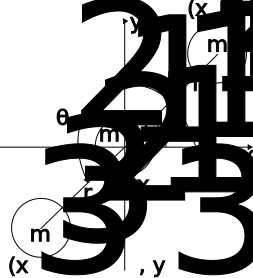
\includegraphics[width=300px]{Three body problem.png}
	\end{figure}
	
	Here we have ignored the third dimension of space, as in many real-life problems bodies move largely in a 2D plane. We will be approaching finding the equations of motion for this system using the \href{https://en.wikipedia.org/wiki/Euler-Lagrange_equations}{Euler-Lagrange equations}:
	
	\begin{align}
		\dfrac{d}{dt}\dfrac{\partial \mathcal{L}}{\partial \dot{q}_i} - \dfrac{\partial \mathcal{L}}{\partial q_i} &= 0.\label{ELE}
	\end{align}
	
	And \href{https://en.wikipedia.org/wiki/Hamilton's_equations}{Hamilton's equations}:
	
	\begin{align}
		\dot{q}_i &= \dfrac{\partial \mathcal{H}}{\partial p_i} \\
		\dot{p}_i &= -\dfrac{\partial \mathcal{H}}{\partial q_i}.
	\end{align}
	
	\tableofcontents
	
	\section{Centred first mass -- Cartesian coordinates}
	\subsection{Velocities and distances}
	In this diagram, we have our axes centred on the first body (whose mass is $m_1$). Hence $x_1=y_1 = 0$ and $\dot{x}_1 = \dot{y}_1 = 0$. Hence the square of $m_2$ and $m_3$'s velocity relative to our axes is: 
	\begin{align*}
		v_2^2 &= \dot{x}_2^2 + \dot{y}_2^2 \\
		v_3^2 &= \dot{x}_3^2 + \dot{y}_3^2.
	\end{align*}
	
	Next we will calculate the distance between the centre of our masses as this is required to calculate the gravitational potential energy. Let $|\vec{r}_{ij}|$ denote the distance between bodies $i$ and $j$. 
	
	\begin{align*}
		\left|\vec{r}_{12}\right| &= \sqrt{x_2^2+y_2^2} \\
		\left|\vec{r}_{13}\right| &= \sqrt{x_3^2+y_3^2} \\
		\left|\vec{r}_{23}\right| &= \sqrt{(x_3-x_2)^2+(y_3-y_2)^2}.
	\end{align*}
	
	\subsection{Kinetic energies}
	
	The kinetic energies of the two bodies in motion are:
	
	\begin{align*}
		T_2 &= \dfrac{m_2}{2} v_2^2 \\
		&= \dfrac{m_2}{2} \left(\dot{x}_2^2 + \dot{y}_2^2\right). \\
		T_3 &= \dfrac{m_3}{2}v_3^2 \\
		&= \dfrac{m_3}{2} \left(\dot{x}_3^2 + \dot{y}_3^2\right).
	\end{align*}
	
	Hence the total kinetic energy of the system is:
	
	\begin{align*}
		T &= T_2 + T_3 \\
		&= \dfrac{m_2}{2} \left(\dot{x}_2^2 + \dot{y}_2^2\right) + \dfrac{m_3}{2} \left(\dot{x}_3^2 + \dot{y}_3^2\right)
	\end{align*}
	
	\subsection{Potential energy}
	The gravitational potential energy is:
	
	\begin{align*}
		V_{12} &= -\dfrac{Gm_1m_2}{|\vec{r}_{12}|} \\
		&= -\dfrac{Gm_1m_2}{\sqrt{x_2^2+y_2^2}}\\
		V_{13} &= -\dfrac{Gm_1m_3}{|\vec{r}_{13}|} \\
		&= -\dfrac{Gm_1 m_3}{\sqrt{x_3^2+y_3^2}} \\
		V_{23} &= -\dfrac{Gm_2m_3}{|\vec{r}_{23}|} \\
		&= -\dfrac{Gm_2 m_3}{\sqrt{(x_3-x_2)^2+(y_3-y_2)^2}} \\
		V &= \sum_{i,j} V_{ij} \\
		&= V_{12}+V_{13} +V_{23} \\
		&= -G\left[\dfrac{m_1m_2}{\sqrt{x_2^2+y_2^2}} + \dfrac{m_1 m_3}{\sqrt{x_3^2+y_3^2}} + \dfrac{m_2 m_3}{\sqrt{(x_3-x_2)^2+(y_3-y_2)^2}}\right].
	\end{align*}
	
	\subsection{Lagrangian}
	Hence the Lagrangian is:
	
	\begin{align*}
		\mathcal{L} &= T - V \\
		&= \dfrac{m_2}{2} \left(\dot{x}_2^2 + \dot{y}_2^2\right) + \dfrac{m_3}{2} \left(\dot{x}_3^2 + \dot{y}_3^2\right) + G\left[\dfrac{m_1m_2}{\sqrt{x_2^2+y_2^2}} + \dfrac{m_1 m_3}{\sqrt{x_3^2+y_3^2}} + \dfrac{m_2 m_3}{\sqrt{(x_3-x_2)^2+(y_3-y_2)^2}}\right].\\
	\end{align*}
	
	\subsection{Euler-Lagrange equations}
	\subsubsection{$x_2$}
	First we calculate the generalized momentum and its time derivative:
	\begin{align*}
		p_{x_2} &= \dfrac{\partial \mathcal{L}}{\partial \dot{x}_2} \\
		&= m_2 \dot{x}_2 \\
		\dot{p}_{x_2} &= m_2 \ddot{x}_2.
	\end{align*}
	Next we calculate:
	
	\begin{align*}
		F_{x_2} &= \dfrac{\partial \mathcal{L}}{\partial x_2} \\
		&= -\dfrac{Gm_1 m_2x_2}{\left(x_2^2+y_2^2\right)^{3/2}} -\dfrac{Gm_2m_3(x_2-x_3)}{\left((x_3-x_2)^2+(y_3-y_2)^2\right)^{3/2}}.
	\end{align*}
	
	Equation \eqref{ELE} hence becomes:
	
	\begin{align*}
		\dot{p}_{x_2} - F_{x_2} &= 0\\
		m_2 \ddot{x}_2 - \left(-\dfrac{Gm_1 m_2x_2}{\left(x_2^2+y_2^2\right)^{3/2}} -\dfrac{Gm_2m_3(x_2-x_3)}{\left((x_3-x_2)^2+(y_3-y_2)^2\right)^{3/2}}\right) &= 0 \\
		m_2 \ddot{x}_2 + \dfrac{Gm_1 m_2x_2}{\left(x_2^2+y_2^2\right)^{3/2}} +\dfrac{Gm_2m_3(x_2-x_3)}{\left((x_3-x_2)^2+(y_3-y_2)^2\right)^{3/2}} &= 0
	\end{align*}
	Dividing by $m_2$ yields and subtracting $\dfrac{Gm_1 m_2x_2}{\left(x_2^2+y_2^2\right)^{3/2}} +\dfrac{Gm_2m_3(x_2-x_3)}{\left((x_3-x_2)^2+(y_3-y_2)^2\right)^{3/2}}$ from both sides yields:
	
	\begin{align*}
		\ddot{x}_2 &= -\dfrac{Gm_1x_2}{\left(x_2^2+y_2^2\right)^{3/2}} -\dfrac{Gm_3(x_2-x_3)}{\left((x_3-x_2)^2+(y_3-y_2)^2\right)^{3/2}}.
	\end{align*}
	
	\subsubsection{$y_2$}
	Our equations are symmetric about $x$ and $y$ coordinates, so the equation for $y_2$ should be:
	
	\begin{align*}
		\ddot{y}_2 &= -\dfrac{Gm_1y_2}{\left(x_2^2+y_2^2\right)^{3/2}} -\dfrac{Gm_3(y_2-y_3)}{\left((x_3-x_2)^2+(y_3-y_2)^2\right)^{3/2}}
	\end{align*}
	
	\subsubsection{$x_3$}
	Our equations are also fairly symmetric about the body under study. So $x_3$'s equation should be similar to that of $x_2$:
	
	\begin{align*}
		\ddot{x}_3 &= -\dfrac{Gm_1x_3}{\left(x_3^2+y_3^2\right)^{3/2}} -\dfrac{Gm_2(x_3-x_2)}{\left((x_3-x_2)^2+(y_3-y_2)^2\right)^{3/2}}.
	\end{align*}
	
	\subsubsection{$y_3$}
	Utilizing symmetry again, yields:
	
	\begin{align*}
		\ddot{y}_3 &= -\dfrac{Gm_1y_3}{\left(x_3^2+y_3^2\right)^{3/2}} -\dfrac{Gm_2(y_3-y_2)}{\left((x_3-x_2)^2+(y_3-y_2)^2\right)^{3/2}}.
	\end{align*}
	
	\subsection{Hamiltonian}
	By symmetry:
	\begin{align*}
		p_{x_2} &= m_2 \dot{x}_2 & p_{y_2} &= m_2 \dot{y}_2\\
		p_{x_3} &= m_3 \dot{x}_3 & p_{y_3} &= m_3 \dot{y}_3.
	\end{align*}
	Hence:
	
	\begin{align*}
		T &= \dfrac{p_{x_2}^2 + p_{y_2}^2}{2m_2} + \dfrac{p_{x_3}^2 + p_{y_3}^2}{2m_3}.
	\end{align*}
	
	Which means the Hamiltonian is:
	
	\begin{align*}
		\mathcal{H} &= \dfrac{p_{x_2}^2 + p_{y_2}^2}{2m_2} + \dfrac{p_{x_3}^2 + p_{y_3}^2}{2m_3} -G\left[\dfrac{m_1m_2}{\sqrt{x_2^2+y_2^2}} + \dfrac{m_1 m_3}{\sqrt{x_3^2+y_3^2}} + \dfrac{m_2 m_3}{\sqrt{(x_3-x_2)^2+(y_3-y_2)^2}}\right].
	\end{align*}
	The Hamiltonian is separable into a kinetic energy term that depends on momenta only and a potential that depends on generalized coordinates only. Consequently, it can be integrated using symplectic integrators such as Yoshida's 4th-order method. 
	
	\subsection{Hamilton's equations}
	Hamilton's equations for spatial coordinate time derivatives are therefore:
	
	\begin{align*}
		\dot{x}_2 &= \dfrac{\partial \mathcal{H}}{\partial p_{x_2}} & \dot{y}_2 &= \dfrac{\partial \mathcal{H}}{\partial p_{y_2}} \\
		&= \dfrac{p_{x_2}}{m_2} & &= \dfrac{p_{y_2}}{m_2} \\
		\dot{x}_3 &= \dfrac{\partial \mathcal{H}}{\partial p_{x_3}} & \dot{y}_3 &= \dfrac{\partial \mathcal{H}}{\partial p_{y_3}} \\
		&= \dfrac{p_{x_3}}{m_3} & &= \dfrac{p_{y_3}}{m_3}
	\end{align*}
	
	As for the time derivatives of momenta:
	\begin{align*}
		\dot{p}_{x_2} &= -\dfrac{\partial \mathcal{H}}{\partial x_2} \\
		&= -\left[-\dfrac{-\dfrac{1}{2}Gm_1m_2 \cdot 2x_2}{(x_2^2+y_2^2)^{3/2}} - \dfrac{-\dfrac{1}{2}Gm_2m_3 \cdot 2(x_3-x_2)\cdot -1}{((x_3-x_2)^2+(y_3-y_2)^2)^{3/2}}\right] \\
		&= -\dfrac{Gm_1m_2x_2}{(x_2^2+y_2^2)^{3/2}} - \dfrac{Gm_2m_3(x_2-x_3)}{((x_3-x_2)^2+(y_3-y_2)^2)^{3/2}} \\
		&= -Gm_2\left[\dfrac{m_1x_2}{(x_2^2+y_2^2)^{3/2}} + \dfrac{m_3(x_2-x_3)}{((x_3-x_2)^2+(y_3-y_2)^2)^{3/2}}\right]\\
		\dot{p}_{y_2} &= -Gm_2\left[\dfrac{m_1y_2}{(x_2^2+y_2^2)^{3/2}} + \dfrac{m_3(y_2-y_3)}{((x_3-x_2)^2+(y_3-y_2)^2)^{3/2}}\right]\\
		\dot{p}_{x_3} &= -Gm_3\left[\dfrac{m_1x_3}{(x_3^2+y_3^2)^{3/2}} + \dfrac{m_2(x_3-x_2)}{((x_3-x_2)^2+(y_3-y_2)^2)^{3/2}}\right]\\
		\dot{p}_{y_3} &= -Gm_3\left[\dfrac{m_1y_3}{(x_3^2+y_3^2)^{3/2}} + \dfrac{m_2(y_3-y_2)}{((x_3-x_2)^2+(y_3-y_2)^2)^{3/2}}\right]
	\end{align*}
	
	\section{Centred first mass -- polar coordinates}
	\subsection{Positions, velocities and distances}
	\begin{align*}
		x_2 &= r_1 \cos{\theta_1} & y_2 &= r_1 \sin{\theta_1}\\
		x_3 &= r_2 \cos{\theta_2} & y_3 &= rt_2 \sin{\theta_2} \\
		\dot{x}_2 &= \dot{r}_1 \cos{\theta_1} - r_1 \dot{\theta}_1 \sin{\theta_1} & \dot{y}_2 &= \dot{r}_1 \sin{\theta_1} + r_1 \dot{\theta}_1 \cos{\theta_1} \\
		\dot{x}_3 &= \dot{r}_2 \cos{\theta_2} - r_2 \dot{\theta}_2 \sin{\theta_2} & \dot{y}_3 &= \dot{r}_2 \sin{\theta_2} + r_2 \dot{\theta}_2 \cos{\theta_2}.
	\end{align*}
	
	Hence the square of the velocities are:
	\begin{align*}
		v_2^2 &= \dot{x}_2^2 + \dot{y}_2^2 & v_3^2 &= \dot{x}_3^2 + \dot{y}_3^2\\
		&= (\dot{r}_1 \cos{\theta_1} - r_1 \dot{\theta}_1 \sin{\theta_1})^2 + (\dot{r}_1 \sin{\theta_1} + r_1 \dot{\theta}_1 \cos{\theta_1})^2 & &= \dot{r}_2^2 + r_2^2 \dot{\theta}_2^2.\\
		&= \dot{r}_1^2 + r_1^2 \dot{\theta}_1^2.
	\end{align*}
	
	As for the distance between masses 2 and 3, it is:
	
	\begin{align*}
		\left|\Delta \vec{r}_{23}\right| &= \left|(r_1\cos{\theta_1} - r_2\cos{\theta_2}, r_1\sin{\theta_1} - r_2\sin{\theta_2})\right| \\
		&= \sqrt{(r_1\cos{\theta_1} - r_2\cos{\theta_2})^2+(r_1\sin{\theta_1} - r_2\sin{\theta_2})^2} \\
		&= \sqrt{r_1^2 + r_2^2 - 2r_1 r_2 \cos{(\theta_2-\theta_1)}}.
	\end{align*}
	
	\subsection{Kinetic energy}
	\begin{align*}
		T &= \dfrac{m_2v_2^2}{2}  + \dfrac{m_3v_3^2}{2} \\
		&= \dfrac{m_2}{2} (\dot{r}_1^2 + r_1^2 \dot{\theta}_1^2) + \dfrac{m_3}{2}(\dot{r}_2^2 + r_2^2 \dot{\theta}_2^2).
	\end{align*}
	
	\subsection{Potential energy}
	\begin{align*}
		V &= -\dfrac{Gm_1m_2}{r_1} - \dfrac{Gm_1m_3}{r_2} - \dfrac{Gm_2 m_3}{\sqrt{r_1^2 + r_2^2 - 2r_1 r_2 \cos{(\theta_2-\theta_1)}}}.
	\end{align*}
	
	\subsection{Lagrangian}
	\begin{align*}
		\mathcal{L} &= \dfrac{m_2}{2} (\dot{r}_1^2 + r_1^2 \dot{\theta}_1^2) + \dfrac{m_3}{2}(\dot{r}_2^2 + r_2^2 \dot{\theta}_2^2) + \dfrac{Gm_1m_2}{r_1} + \dfrac{Gm_1m_3}{r_2} + \dfrac{Gm_2 m_3}{\sqrt{r_1^2 + r_2^2 - 2r_1 r_2 \cos{(\theta_2-\theta_1)}}}.
	\end{align*}
	
	\subsection{Euler-Lagrange equations}
	\subsubsection{$r_1$}
	\begin{align*}
		p_{r_1} &= \dfrac{\partial \mathcal{L}}{\partial \dot{r}_1} & F_{r_1} &= \dfrac{\partial \mathcal{L}}{\partial r_1} \\
		&= m_2\dot{r}_1 & &= m_2 r_1\dot{\theta}_1^2 \\
		\dot{p}_{r_1} &= m_2\ddot{r}_1.
	\end{align*}
	
	Hence the Euler-Lagrange equation for $r_1$ is:
	
	\begin{align*}
		m_2\ddot{r}_1 - m_2 r_1\dot{\theta}_1^2 &= 0 \\
		\ddot{r}_1 - r_1 \dot{\theta}_1^2 &= 0 \\
		\ddot{r}_1 &= r_1 \dot{\theta}_1^2.
	\end{align*}
		
	\subsubsection{$r_2$}
	\begin{align*}
		p_{r_2} &= \dfrac{\partial \mathcal{L}}{\partial \dot{r}_2} & F_{r_2} &= \dfrac{\partial \mathcal{L}}{\partial r_2} \\
		&= m_3\dot{r}_2 & &= m_3 r_2\dot{\theta}_2^2\\
		\dot{p}_{r_2} &= m_3\ddot{r}_2.
	\end{align*}
	Hence the Euler-Lagrange equation for $r_2$ is:
	\begin{align*}
		m_3 \ddot{r}_2 - m_3 r_2 \dot{\theta}_2^2 &= 0 \\
		\ddot{r}_2 - r_2 \dot{\theta}_2^2 &= 0 \\
		\ddot{r}_2 &= r_2 \dot{\theta}_2^2.
	\end{align*}
	
	\subsubsection{$\theta_1$}
	\begin{align*}
		p_{\theta_1} &= \dfrac{\partial \mathcal{L}}{\partial \dot{\theta}_1} & F_{\theta_1} &= \dfrac{\partial \mathcal{L}}{\partial \theta_1}\\
		&= m_2 r_1^2 \dot{\theta}_1 & &= \dfrac{Gm_2 m_3\cdot-\dfrac{1}{2}\cdot (-2r_1r_2\cdot -\sin{(\theta_2-\theta_1)\cdot -1})}{(r_1^2 + r_2^2 - 2r_1 r_2 \cos{(\theta_2-\theta_1)})^{3/2}} \\
		\dot{p}_{\theta_1} &= 2m_2 r_1\dot{r}_1 \dot{\theta}_1 + m_2 r_1^2 \ddot{\theta}_1 & &= \dfrac{Gm_2 m_3 r_1 r_2 \sin{(\theta_2-\theta_1)}}{(r_1^2 + r_2^2 - 2r_1 r_2 \cos{(\theta_2-\theta_1)})^{3/2}}.
	\end{align*}
	Hence the Euler-Lagrange equation for $\theta_1$ is:
	\begin{align*}
		2m_2 r_1\dot{r}_1 \dot{\theta}_1 + m_2 r_1^2 \ddot{\theta}_1 - \dfrac{Gm_2 m_3 r_1 r_2 \sin{(\theta_2-\theta_1)}}{(r_1^2 + r_2^2 - 2r_1 r_2 \cos{(\theta_2-\theta_1)})^{3/2}} &= 0 \\
		\dfrac{2\dot{r}_1 \dot{\theta}_1}{r_1} + \ddot{\theta}_1 - \dfrac{Gm_3r_2\sin{(\theta_2-\theta_1)}}{r_1(r_1^2 + r_2^2 - 2r_1 r_2 \cos{(\theta_2-\theta_1)})^{3/2}} &= 0\\
		\ddot{\theta}_1 &= -\dfrac{2\dot{r}_1 \dot{\theta}_1}{r_1} + \dfrac{Gm_3r_2\sin{(\theta_2-\theta_1)}}{r_1(r_1^2 + r_2^2 - 2r_1 r_2 \cos{(\theta_2-\theta_1)})^{3/2}}.
	\end{align*}
	
	\subsubsection{$\theta_2$}
	\begin{align*}	
		p_{\theta_2} &= \dfrac{\partial \mathcal{L}}{\partial \dot{\theta}_2} & F_{\theta_2} &= \dfrac{\partial \mathcal{L}}{\partial \theta_2}\\
		&= m_3 r_2^2 \dot{\theta}_2 & &= \dfrac{Gm_2m_3\cdot -\dfrac{1}{2} \cdot (-2r_1r_2 \cdot -\sin{(\theta_1-\theta_2)\cdot -1})}{(r_1^2 + r_2^2 - 2r_1 r_2 \cos{(\theta_2-\theta_1)})^{3/2}}\\
		\dot{p}_{\theta_2} &= 2m_3 r_2 \dot{r}_2 \dot{\theta}_2 + m_3r_2^2 \ddot{\theta}_2 & &= \dfrac{Gm_2m_3r_1r_2 \sin{(\theta_1-\theta_2)}}{(r_1^2 + r_2^2 - 2r_1 r_2 \cos{(\theta_2-\theta_1)})^{3/2}}
	\end{align*}
	Hence the Euler-Lagrange equation for $\theta_2$ is:
	\begin{align*}
		2m_3 r_2 \dot{r}_2 \dot{\theta}_2 + m_3r_2^2 \ddot{\theta}_2 - \dfrac{Gm_2m_3r_1r_2 \sin{(\theta_1-\theta_2)}}{(r_1^2 + r_2^2 - 2r_1 r_2 \cos{(\theta_2-\theta_1)})^{3/2}} &= 0 \\
		\dfrac{2\dot{r}_2 \dot{\theta}_2}{r_2} + \ddot{\theta}_2 - \dfrac{Gm_2r_1\sin{(\theta_1-\theta_2)}}{r_2(r_1^2 + r_2^2 - 2r_1 r_2 \cos{(\theta_2-\theta_1)})^{3/2}} &= 0\\
		\ddot{\theta}_2 &= -\dfrac{2\dot{r}_2 \dot{\theta}_2}{r_2} + \dfrac{Gm_2r_1\sin{(\theta_1-\theta_2)}}{r_2(r_1^2 + r_2^2 - 2r_1 r_2 \cos{(\theta_2-\theta_1)})^{3/2}}.
	\end{align*}
	\subsection{Hamiltonian}
	Rewriting the kinetic energy in terms of the canonical momenta:
	
	\begin{align*}
		T &= \dfrac{p_{r_1}^2}{2m_2}+\dfrac{p_{\theta_1}^2}{2m_2r_1^2} + \dfrac{p_{r_2}^2}{2m_3}+\dfrac{p_{\theta_2}^2}{2m_3r_2^2}.
	\end{align*}
	
	Hence the Hamiltonian is:
	
	\begin{align*}
		\mathcal{H} &= \dfrac{p_{r_1}^2}{2m_2}+\dfrac{p_{\theta_1}^2}{2m_2r_1^2} + \dfrac{p_{r_2}^2}{2m_3}+\dfrac{p_{\theta_2}^2}{2m_3r_2^2} -\dfrac{Gm_1m_2}{r_1} - \dfrac{Gm_1m_3}{r_2} - \dfrac{Gm_2 m_3}{\sqrt{r_1^2 + r_2^2 - 2r_1 r_2 \cos{(\theta_2-\theta_1)}}}.
	\end{align*}
	\subsection{Hamilton's equations}
	\subsubsection{$r_1$}
	\begin{align*}
		\dot{r}_1 &= \dfrac{\partial \mathcal{H}}{\partial p_{r_1}} & \dot{p}_{r_1} &= -\dfrac{\partial \mathcal{H}}{\partial r_1} \\
		&= \dfrac{p_{r_1}}{m_2} & &=-\left[ -\dfrac{2p_{\theta_1}^2}{2m_2r_1^3} - \dfrac{Gm_1m_2\cdot -1}{r_1^2} - \dfrac{Gm_2m_3\cdot -\dfrac{1}{2} \cdot(2r_1-2r_2\cos{(\theta_2-\theta_1)})}{(r_1^2 + r_2^2 - 2r_1 r_2 \cos{(\theta_2-\theta_1)})^{3/2}} \right]\\
		&& &= \dfrac{p_{\theta_1}^2}{m_2r_1^3} - \dfrac{Gm_1m_2}{r_1^2} - \dfrac{Gm_2m_3(r_1-r_2\cos{(\theta_2-\theta_1)})}{(r_1^2 + r_2^2 - 2r_1 r_2 \cos{(\theta_2-\theta_1)})^{3/2}}.
	\end{align*}
	\subsection{$r_2$}
	\begin{align*}
		\dot{r}_2 &= \dfrac{\partial \mathcal{H}}{\partial p_{r_2}} & \dot{p}_{r_2} &= -\dfrac{\partial \mathcal{H}}{\partial r_2}\\
		&= \dfrac{p_{r_2}}{m_3} & &= -\left[-\dfrac{2p_{\theta_2}^2}{2m_3r_2^3} - \dfrac{Gm_1m_3\cdot-1}{r_2^2} - \dfrac{Gm_2m_3 \cdot -\dfrac{1}{2}\cdot (2r_2 -2r_1\cos{(\theta_2-\theta_1)})}{(r_1^2 + r_2^2 - 2r_1 r_2 \cos{(\theta_2-\theta_1)})^{3/2}}\right] \\
		& & &= \dfrac{p_{\theta_2}^2}{m_3r_2^3} - \dfrac{Gm_1m_3}{r_2^2} - \dfrac{Gm_2m_3(r_2-r_1\cos{(\theta_2-\theta_1)})}{(r_1^2 + r_2^2 - 2r_1 r_2 \cos{(\theta_2-\theta_1)})^{3/2}}.
	\end{align*}
	\subsection{$\theta_1$}
	\begin{align*}
		\dot{\theta}_1 &= \dfrac{\partial \mathcal{H}}{\partial p_{\theta_1}} & \dot{p}_{\theta_1} &= -\dfrac{\partial \mathcal{H}}{\partial \theta_1} \\
		&= \dfrac{p_{\theta_1}}{m_2r_1^2} & &=-\left[-\dfrac{Gm_2m_3\cdot -\dfrac{1}{2} \cdot -2r_1r_2\cdot -\sin{(\theta_2-\theta_1)}\cdot -1}{(r_1^2 + r_2^2 - 2r_1 r_2 \cos{(\theta_2-\theta_1)})^{3/2}}\right] \\
		& & &= \dfrac{Gm_2m_3r_1r_2 \sin{(\theta_2-\theta_1)}}{(r_1^2 + r_2^2 - 2r_1 r_2 \cos{(\theta_2-\theta_1)})^{3/2}}
	\end{align*}
	\subsection{$\theta_2$}
	\begin{align*}
		\dot{\theta}_2 &= \dfrac{\partial \mathcal{H}}{\partial p_{\theta_2}} & \dot{p}_{\theta_2} &= -\dfrac{\partial \mathcal{H}}{\partial \theta_2} \\
		&= \dfrac{p_{\theta_2}}{m_3r_2^2} & &= -\left[-\dfrac{Gm_2m_3\cdot -\dfrac{1}{2} \cdot -2r_1r_2 \cdot -\sin{(\theta_2-\theta_1)}\cdot 1}{(r_1^2 + r_2^2 - 2r_1 r_2 \cos{(\theta_2-\theta_1)})^{3/2}}\right] \\
		& & &=\dfrac{Gm_2m_3 r_1r_2 \sin{(\theta_1-\theta_2)}}{(r_1^2 + r_2^2 - 2r_1 r_2 \cos{(\theta_2-\theta_1)})^{3/2}}.
	\end{align*}
\end{document}